\documentclass[11pt,a4paper,titlepage]{article}

\usepackage[top=2.5cm,left=1.5cm,right=1.5cm,bottom=2cm,headheight=13.6cm]{geometry}
\usepackage{color}
\usepackage{listings}
\usepackage[font=small,labelfont=bf]{caption} % figure caption
\usepackage{subcaption}
\usepackage{float}
\usepackage{titling}
\usepackage{amsmath} % cases
\usepackage{multicol}
\usepackage{xltxtra}
\usepackage{siunitx}
\usepackage{csvsimple}
\usepackage[nottoc,numbib]{tocbibind}
\usepackage[normalem]{ulem}
\usepackage[table,xcdraw]{xcolor}
\usepackage{fontspec} % set truetype font
\usepackage{pgfkeys}
\usepackage{soul} % fancy underlining
\usepackage{cite} % for range e.g [1-3]

%unicode fixer
%\usepackage[Latin,Greek,Phonetics]{ucharclasses} % please make unicode work. Please.
%\newfontfamily\substitutefont{Iosevka} % has most glyphs 
%\setTransitionsFor{IPAExtensions}{\begingroup\substitutefont}{\endgroup}

\setmonofont[Scale=MatchLowercase]{Iosevka}

% restore sensible table spacings
\renewcommand{\arraystretch}{1.5}

\definecolor{mygreen}{RGB}{0,127,0}
\definecolor{mygray}{RGB}{100,100,100}
\definecolor{mymauve}{RGB}{100,32,255}
\definecolor{lgray}{RGB}{230,230,230}
\settocbibname{Bibliography}
\lstset{ %
  frame=none,
  backgroundcolor=\color{white},   % choose the background color; you must add \usepackage{color} or \usepackage{xcolor}
  basicstyle=\footnotesize\ttfamily,        % the size of the fonts that are used for the code
  breakatwhitespace=false,         % sets if automatic breaks should only happen at whitespace
  breaklines=true,                 % sets automatic line breaking
  captionpos=t,                    % sets the caption-position to bottom
  commentstyle=\color{mygreen},    % comment style
  deletekeywords={...},            % if you want to delete keywords from the given language
  escapeinside={\%*}{*)},          % if you want to add LaTeX within your code
  extendedchars=true,              % lets you use non-ASCII characters; for 8-bits encodings only, does not work with UTF-8
%  frame=single,                    % adds a frame around the code
  keepspaces=true,                 % keeps spaces in text, useful for keeping indentation of code (possibly needs columns=flexible)
  keywordstyle=\color{blue},       % keyword style
  language=,                 % the language of the code
  morekeywords={*,...},            % if you want to add more keywords to the set
  numbers=left,                    % where to put the line-numbers; possible values are (none, left, right)
  numbersep=5pt,                   % how far the line-numbers are from the code
  numberstyle=\tiny\color{mygray}, % the style that is used for the line-numbers
  rulecolor=\color{black},         % if not set, the frame-color may be changed on line-breaks within not-black text (e.g. comments (green here))
  showspaces=false,                % show spaces everywhere adding particular underscores; it overrides 'showstringspaces'
  showstringspaces=false,          % underline spaces within strings only
  showtabs=false,                  % show tabs within strings adding particular underscores
  stepnumber=1,                    % the step between two line-numbers. If it's 1, each line will be numbered
  stringstyle=\color{mymauve},     % string literal style
  tabsize=4,                       % sets default tabsize to 2 spaces
  aboveskip=3mm,
  belowskip=3mm,
}

\usepackage{fancyhdr}
\usepackage{datetime}
\usepackage{moresize}
\usepackage{titlesec}
%  Clickable TOC and refs
\usepackage{hyperref}
\hypersetup{
    colorlinks,
    citecolor=black,
    filecolor=black,
    linkcolor=black,
    urlcolor=black
}
% Fix fonts in TOC
\usepackage{tocloft}

\pagestyle{fancy}
\rhead{\lightfont Y3761870}
\renewcommand{\headrulewidth}{2pt}% 2pt header rule
\renewcommand{\headrule}{\hbox to\headwidth{%
 \color{lgray}\leaders\hrule height \headrulewidth\hfill}}

% table of contents depth
\setcounter{tocdepth}{2}
  
\setsansfont{DINPro-Bold.otf}
\newfontfamily\boldfont{DINPro-Bold.otf}
\newfontfamily\mediumfont{DINPro-Medium.otf}
\newfontfamily\regularfont{DINPro-Regular.otf}
\newfontfamily\lightfont{DINPro-Light.otf}
%\newfontfamily\ttfamily{iosevka-custom-regular.ttf} % too big
% Set formats for each heading level
\titleformat*{\section}{\Large\bfseries\sffamily}
\titleformat*{\subsection}{\large\bfseries\mediumfont}
\titleformat*{\subsubsection}{\itshape\mediumfont}

\renewcommand{\contentsname}{C O N T E N T S}
\renewcommand{\cfttoctitlefont}{\small\regularfont\MakeUppercase}
\renewcommand{\cftsecfont}{\regularfont}
\renewcommand{\cftsecpagefont}{\mediumfont}
\renewcommand{\cftsubsecfont}{\lightfont}
\renewcommand{\cftsubsecpagefont}{\regularfont}
% Adjust spacing in TOC
\setlength\cftbeforesubsecskip{5pt}
% remove annoying space before maths
\setlength{\abovedisplayskip}{0pt}


% redefine footer
\fancyfoot[C]{\regularfont\fontsize{11pt}{11pt}\selectfont\thepage} % except the center


\newdateformat{monthyeardate}{%
  \monthname[\THEMONTH] \THEYEAR}

\newcommand{\rulebreak}{%
	\par%
	\vspace{0.9cm}%
    \noindent\color{lgray}\rule{4cm}{2pt}%
    \color{black}%
    \vspace{1.2cm}%
    \par%
}

\newcommand{\coverpage}[1]{%
	\pagenumbering{gobble}%
	\thispagestyle{empty}%
	\lhead{\lightfont\textsc{#1}}%
    \title{Voice Production \& Synthesis}%
    \author{Y3761870}%
    \newgeometry{left=5cm,bottom=2cm,right=5cm,top=2cm}%
	\begin{center}\hspace{0pt}\vfill%
    \uppercase{\lightfont Department of Electronic Engineering\\
    The University of York}
	\rulebreak%
    {\Large\textbf{\sffamily Voice Production \& Synthesis}}
    
    \vspace{0.5cm}
    {\HUGE\textbf{\textit{\sffamily #1}}\par}
    \vspace{1cm}
    
	\theauthor%
	\par%
	\vspace{0.9cm}%
    \noindent\color{lgray}\rule{4cm}{2pt}\color{black}%
    \vspace{0.45cm}
    \tableofcontents%
	\rulebreak%
    \monthyeardate\today\par
    \hspace{0pt}
	\end{center}%
    \vfill
    \hspace{0pt}
	\pagebreak%
    \restoregeometry%
    \pagenumbering{arabic}%
}

\newcommand{\filename}[1]{%
	\texttt{#1}%
}

\newcommand{\ipa}[1]{%
	\texttt{/#1/}%
}

\renewcommand{\~}{\char`~}

\newcommand*{\obj}[1]{\texttt{[#1]}}
\newcommand*{\msg}[1]{\texttt{[#1(}}


\newcommand*\paths[1]{\lstset{inputpath=#1}\graphicspath{#1}}


\paths{{./assets/}}

\begin{document}

	\coverpage{PureData Source-filter Speech Synthesiser}
	
	\begin{multicols}{2}
	
		\section{Principles of voice synthesis}
		The source-filter theory of speech construction considers voice production as essentially a system of a power source exciting a sound source (the vocal folds), which emit sound through a series of filters (the vocal tract) e.g. the nasal cavity, the mouth and its shape being manipulated, the tongue and its position, and finally radiation from the lips. 

This can be modelled relatively simply with some kind of sound source and the vocal tract transfer function (VTTF). 

In the case of simple implementation with PD the sound source can be modelled with some kind of wave rich in harmonics, e.g. a sawtooth wave or, as we'll see, a more sculpted waveform, and the VTTF as a parallel set of filters.

- Talk about what formants are
- Talk about noise production

Sound can be split into two general categories: voiced sound which involves a repeated waveform with a fundamental and a series of harmonics, and unvoiced sound which can be modelled as noise (discuss splitting of this into frication/aspiration in the model)

Need to discuss how this relates to consonants and vowels

Frication noise in consonants is not white noise, it starts to fall off at about 1kHz and continues to drop roughly linearly until 10kHz when it is approximately zero. \cite{Johnson2003} Fricatives work like turbulence - the sound of a jet of air hitting an obstacle. \cite{Johnson2003}

More general stuff can be referenced from \cite{Howard2008}

Discuss formants as the resonant freqencies of the cavities in the vocal track \cite{Johnson2003}

Source-filter theory of speech construction.

used parallel rather than series/cascade formant synthesis. This makes it easier to preserve correct formant amplitudes  \cite{Liljencrants1995} which makes for easier feedback loop on analysing formants and correcting.

LF-model models differentiated glottal flow rather than real glottal flow.

Revisited LF-model uses a data reduction scheme to adjust parameters using a reduction to a few other control parameters \cite{Fant1995}:

Spectral tilt $F_a = 1/(2\pi T_a)$, alternative to $R_a = T_a/T_0$.

\begin{align}
R_a & = \frac{T_a}{T_0} \\
R_g & = T_0/(2T_p) \\
R_k & = (T_e - T_p)/T_p \\
OQ & = T_e/T_0 = (1+R_k)/(2R_g) \\
R_d &= (T_d/T_0)(1/110) \\
&= (U_0/E_e)/(F_0/110) \\
& \approx (0.5 + 1.2R_k)(R_k/(4R_g) + R_a)/0.11
\end{align}

Use \cite{Gobl1988} for indications of parameters for typical male speakers (e.g. $F_a = \si{700 Hz} $, $R_k = 0.30$ $R_g=1.20$. Notes $E_e$ tends to be stronger for vowels and weaker for consonants. Voiced consonants weaker than vowels. Some limitations on this data: it's gathered from only 3 speakers, all Swedish, and all male. This also demonstrates the impact of prosody on voice source parameters. Notes that decrease of $E_e$ is generally accompanied by an increase of $r_a$ and $r_k$.

Increasing $R_k$ raises level of voice fundamental relative to upper parts of the spectrum. Increasing $R_a$ (and thereby decreasing $F_a$) gives a secondary effect of a relative boost of the fundamental which occurs in breathy phonation. Increasing $R_g$ promotes the level of the second harmonic at the expense of the fundamental. Sonorous voices have relatively high $F_a$ of the order of \si{2000Hz} \cite{Fant1995}

The 'shape parameter' $R_d = (U_0/E_e)(F_0/110)$.  \cite{Fant1995} discusses some statistical relations, cited from  a 1994 publication that I was unable to locate a copy of. \cite{Fant1994}. These are the following predicated values, as they relate to $R_d$, and an estimation of $R_d$ from the geometrical constraints of the LF model:

\begin{align}
R_a & \approx (-1+4.8R_d)/100 \\
R_k  & \approx (22.4 + 11.8R_d)/100 \\
R_d & \approx (1/0.11)(0.5+1.2R_k)(R_k/4R_g+R_a)
\end{align}
The main range of variation is $0.3 < R_d < 2.7$, and the upper range is intended for transitions towards complete abduction as in prepause voice terminations.

Here's an example of the variation from \cite{Fant1995}: "
A pronounced vocal-tract narrowing, as in the [i:] and [y:] and the maximally rounded [u:] and [\sout{u}:], causes a loss of transglottal pressure which modifies the glottal flow pulse towards a greater $R_d$ value and a somewhat lower $E_e$."

Higher $R_d$ is typical of female vs male phonations, but also found in voiced consoants and aspirated vowels vs regular vowels. \cite{Fant1995}

Using 'analysis-by-synthesis' to determine LF model parameters, comparing recorded sound with that of a synthesiser and then adjusting parameters until the spectrograms are close to each-other, this is the approach used. \cite{Fant1995}

Naturalness has been shown to be linked with aspiration noise introduced at higher frequencies in the vowels, and also to the relative strength of the fundamental component (less so in the case of a female voice). \cite{Klatt1990}

On naturalness of the voice, one approach is a small slowly varying $F_0$ pseudorandomness \cite{Klatt1990} (period-to-period flutter) – maybe adjusting the timing parameters of the LF model. The same study discusses a diplophonic double pulsing in whcih pairs of glottal pulses migrate toward one another and the first of the pair is usually attenuated in amplitude. Tends to occur when the fundamental is low (voicing is unstable). (possible further improvement).

Note \cite{Klatt1990} discusses the limitations of adding this pseudorandom flutter to $F_0$, referencing that other efforts have led to a harsh voice quality (Rozsypal and Millar, 1979). They propose a slow quasirandom drift to $F_0$ contour thru FL flutter control parameter. The sum of three slowly varying sine waves. Suggested FL value of 25%

\begin{align}
\Delta F_0 = & (FL/50)(F_0/100)(\sin(2 \pi 12.7t) \\ 
& + \sin(2 \pi 7.1t) + \sin(2 \pi 4.7t) \si{Hz}
\end{align}

\cite{Klatt1990} also discusses naturalness by  mixing an impulse train and noise as the source waveform (Kate et al 1967; Holmes 1973) - specifying a cutoff frequency below which the source consists of harmonics, and above which the source if lat-spectrum noise. also see rothenberg et al (1975) and makhoul et al (1978)

The LF model exploits the (assumed) commutative relationship between the voice source, vocal tract, and lip radiation, to combine the ffects of the voice source and lip radiation into one model. \cite{DelPozo2008}

		
		\section{How the PD patch works}
		This section is focused on the audio properties of the PD patch and the control structures which operate them specifically. In addition to this, many different general-purpose control objects were created to streamline development. A full list is available in appendix \ref{x:glossary}, page \pageref{x:glossary}.
%
\begin{figure}[H]
	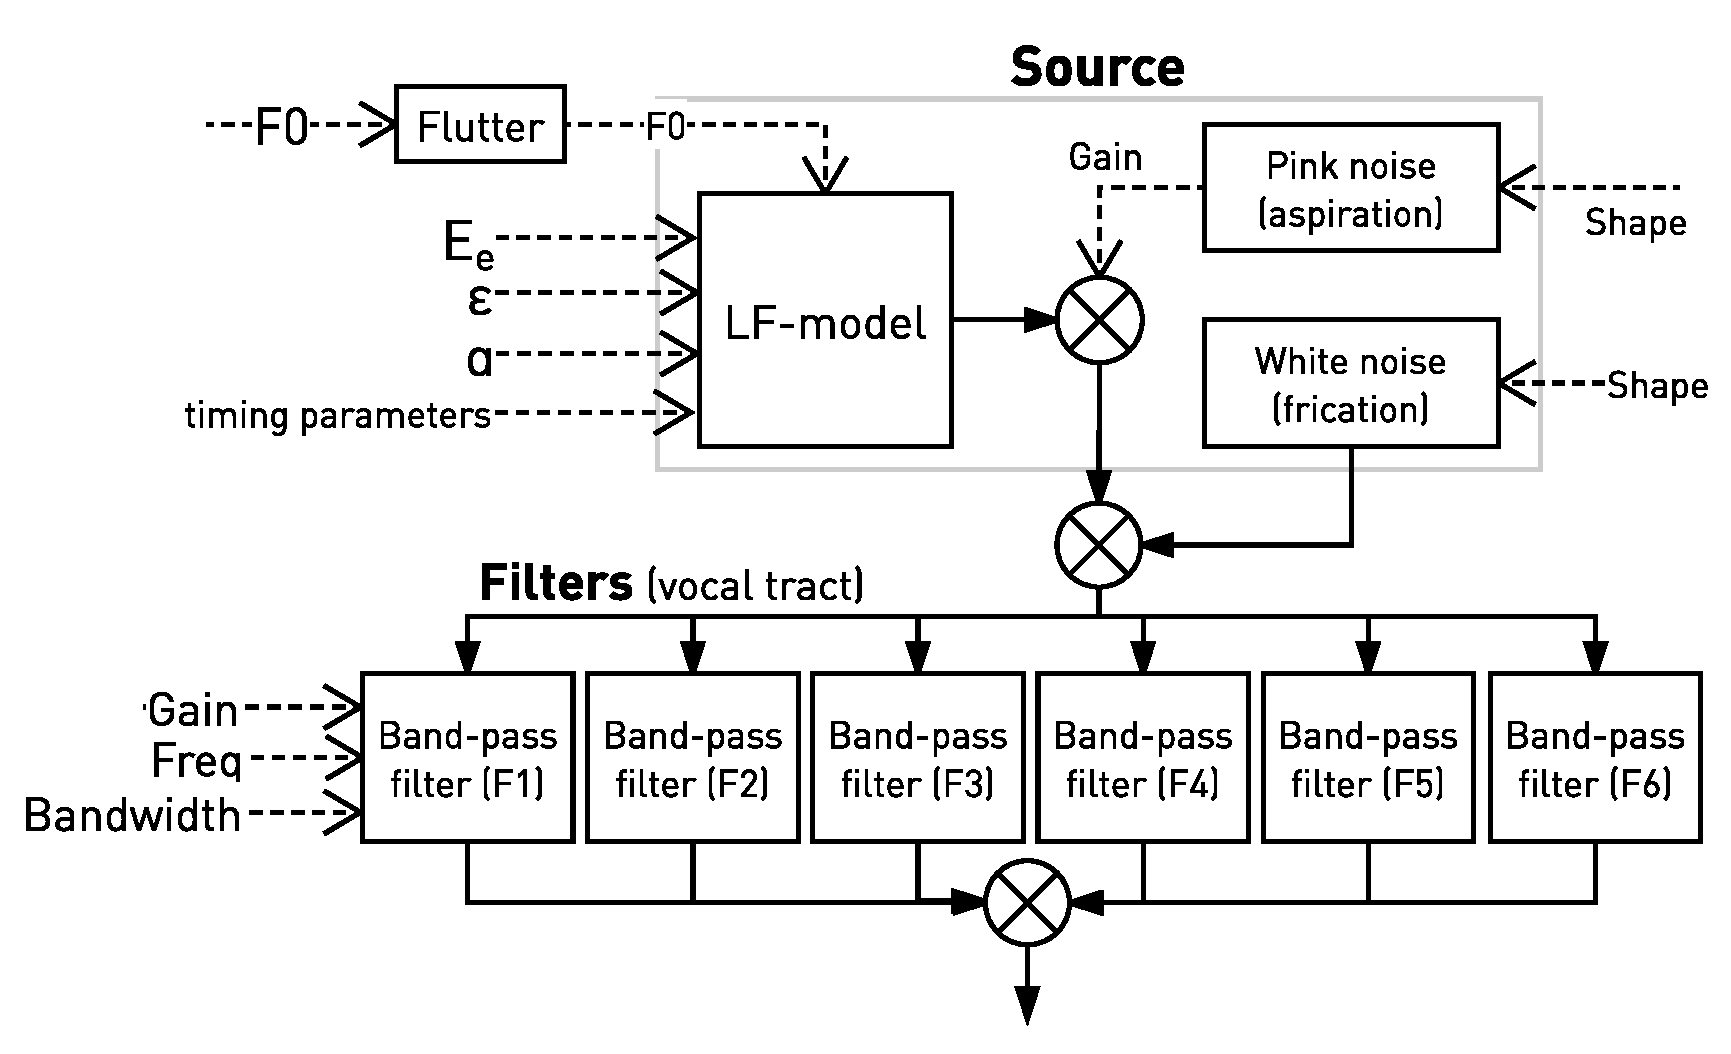
\includegraphics[width=0.5\textwidth]{signal_flow.pdf}
	\caption{Signal path diagram for the system. Audio signals are represented with black arrows, control signals are represented with dotted arrows.}
	\label{fig:signal_path}
\end{figure}
%
The synthesiser is configured as a parallel formant synthesiser with an adjustable LF-model of the glottal flow derivative as the sound source. Aspiration and frication noise are provided by two additional noise generators in the voice source. Pseudo-random flutter is implemented using Klatt's algorithm detailed in the previous section. The formants are modelled as band-pass filters with adjustable gain, centre frequency and bandwidth. The signal path is for this system is outlined in the signal flow diagram in Figure \ref{fig:signal_path} above.

In the top-level patch (\obj{synth}) the connecting edges of the objects are reserved only for audio signals to make the data flow clear (see Figure \ref{fig:top_level} below). Control signals are routed using message receivers.
%
\begin{figure}[H]
	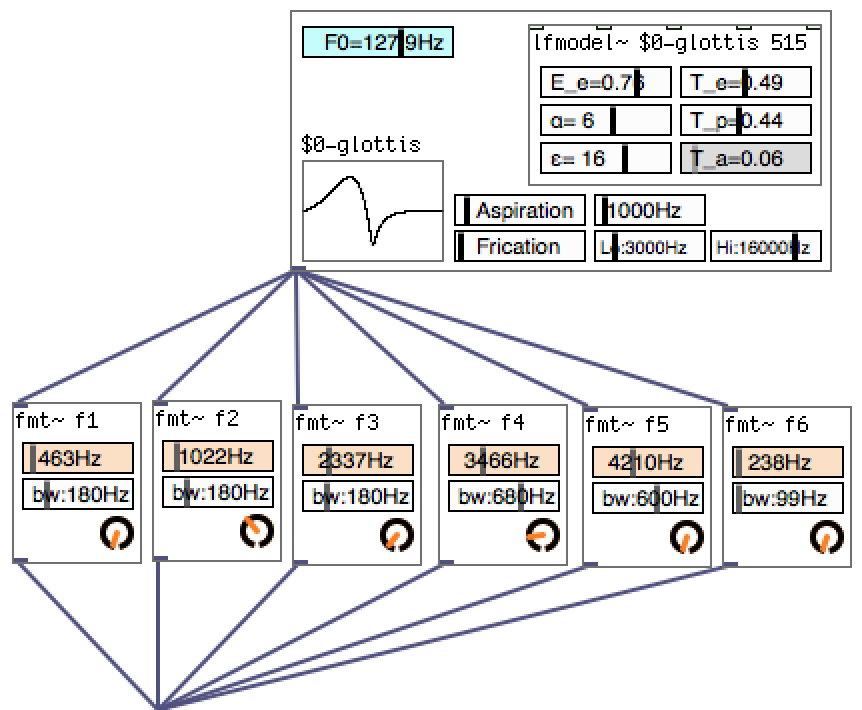
\includegraphics[width=0.5\textwidth]{top_level.png}
	\caption{Signal flow in \obj{synth}: from sound source through the vocal tract.}
	\label{fig:top_level}
\end{figure}
%
I initially used a large number of formants (10). This did create added realism but put a lot of burden when trying to make adjustments. Fant \cite{Fant1995} cites a formula
%
\begin{equation}
	m = F_s(l_e / c)
\end{equation}
%
which defines the minimum number of VTTF poles required to maintain correct spectral distribution for formant synthesis. Assuming an average male vocal tract length of $l_e=17.65\si{5cm}$ and a sampling rate of $F_s = \si{44100Hz}$ this indicates a need for 22 formants. This seems well beyond what is likely to be practical to implement in PD. To determine the resonant frequency of a particular formant Johnson \cite{Johnson2003} gives the formula
%
\begin{equation}
	F_n = \frac{(2n-1)c}{4l_e}
\end{equation}
%
which suggests that the tenth formant comes in at approximately 9.4kHz. As human hearing drops off after 10kHz I see no particular need to implement these higher formants in any case. For simplicity I reduced my system to five formants and added a sixth to model an additional prominent formant movement in the diphthong of my chosen word. I encourage the reader to experiment with selecting the bypass switch on the formants on my patch to hear what difference the formants above $F_3$ make.

In order to recreate the spectrum more precisely I had to use more configurable filters than the standard array of \obj{bp\~}, \obj{lop\~} and \obj{hip\~}. I found for the high and low-pass filters especially that the rolloff was too gradual to be of much use. Instead I used the built-in \obj{biquad\~} filter using \obj{bandpass} to calculate the coefficients for the formants. One problem with this is that if the control parameters are not interpolated smoothly enough it can create artefacts in the synthesis. However, reducing the time-grain for \obj{line} can introduce a lot of processor overhead. I tried to strike a balance. \obj{bandpass} specifies the bandwidth in octaves so I created some logic to convert to a bandwidth in Hertz to make adjustments more quickly. However, it does not map the centre frequency precisely because \obj{bandpass} sets the bandwidth logarithmically rather than linearly. 

A \obj{controller} patch—Figure \ref{fig:controller} below—has any array of buttons for different phonemes and words, and when they are pressed sends control messages to the vocal tract and voice source patches to configure them.
%
\begin{figure}[H] 
	\centering
	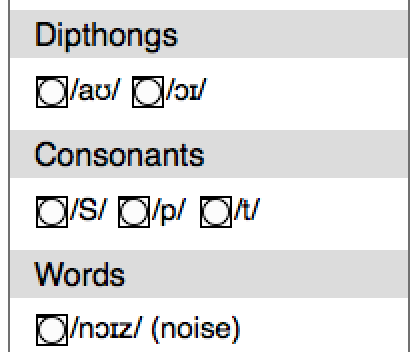
\includegraphics[height=3cm]{controller.png}
	\caption{A small section of the \obj{controller} patch showing how presets can be selected.}
	\label{fig:controller}
\end{figure}
%
Most control messages are terminated with a linear ramp time in ms. Sequencing chains of these events is handled with \obj{qlist} and a message delay pipe, see \obj{msgpipe} in appendix \ref{x:glossary} for more details.

I aimed to create a flexible synthesis system that could be configured rapidly. In the pursuit of naturalness it is equally important to have rapid turnaround of analysis of synthesis attempts, as there is a large element of trial and error without using more sophisticated techniques. To aid with this I created \obj{desk\`} to allow recording directly from the synthesiser as easily as possible (see Figure \ref{fig:desk} below). Once a location has been selected with the `eject' button, pressing record will record to that file until stop is pressed.
%
\begin{figure}[H]
	\centering
	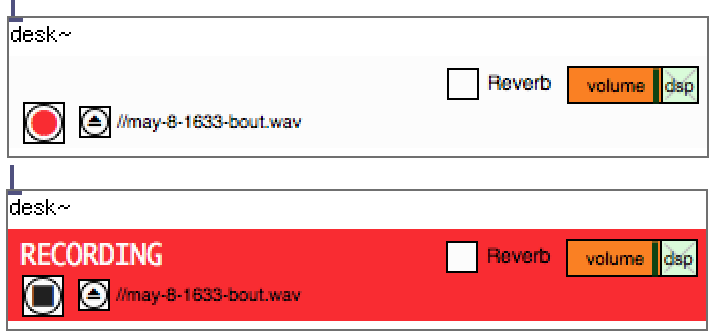
\includegraphics[width=0.39\textwidth]{desk.png}
	\caption{\obj{desk\~} object for rapidly saving samples for analysis when stopped (above) and recording (below).}
	\label{fig:desk}
\end{figure}
%
		
		\section{Critical analysis of the synthesiser}
		Using 'typical' values for voice source parameters is hard because trans voices differ from typical male or female voices. \cite{Gunzburger1995} Particularly for trans women there is a tendency for $F_3$ to be raised compared to male voices, with slower speech at reduced loudness and a higher $F_0$. 

Although the implementation of the LF-model is there I had difficulty utilising it to improve my synthesiser. Determining correct parameters is not trivial as using this `analysis-by-synthesis' approach to compare the synthesised spectrogram with the reference requires a lot of time in a non-automated system such as this PD implementation.

The additional parameters in the revised model \cite{Fant1995} provide further control over the spectrum: increasing $R_k$ raises level of voice fundamental relative to upper parts of the spectrum. Increasing $R_g$ promotes the level of the second harmonic at the expense of the fundamental. This analysis starts to get into the spectral qualities of specific voices, e.g. it is noted that sonorous voices have relatively high $F_a$ of the order of \si{2000Hz} \cite{Fant1995}.

Fant also discusses a shape parameter, $R_d$, which predicts the other values, citing a 1994 publication that I was unable to locate a copy of \cite{Fant1994}. I tried to implement this as I felt it would make it much more straightforward to find appropriate LF-model parameters for my system, however I had enormous problems matching up the ``statistical relations" for the R parameters in the LF-model \cite{Fant1995} - particularly due to an initial misunderstanding of the statistical prediction model. The work in progress for this can be seen in the \obj{lfmodel\char`~} patch. I would very much like to do more research into this and complete the revisited model.

I found that much of my alterations, though making sense from a theoretical perspective and being audible in contrived examples, made minimal impact when real words were being synthesised. It's probably quite important to do real listening tests.

One issue with my system is that the transitions between parameters, e.g. formant centre frequencies, are linear. This isn't actually true to formants in actual speech which have more gradual ramps between positions. See Figure \ref{fig:bout_non_linear_tx} below for an example in an earlier word. For my final word I compensated for this somewhat by having more interpolation points during the word and ramping between them. 
%
\begin{figure}[H] 
	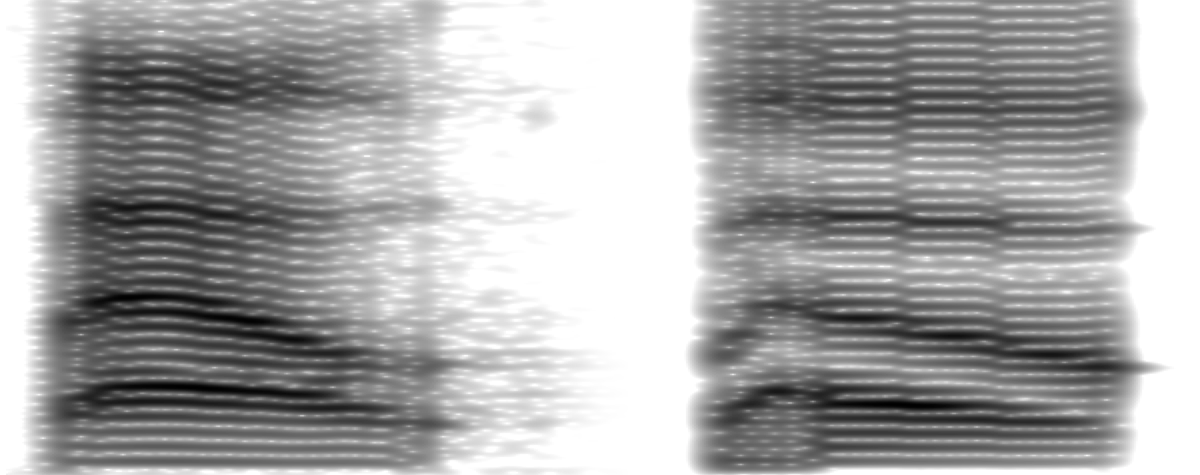
\includegraphics[width=0.5\textwidth]{bout_non_linear_tx.png}
	\caption{Linear vs. non-linear formant transitions of \ipa{baʊt} in the reference recording (left) vs synthesised (right).}
	\label{fig:bout_non_linear_tx}
\end{figure}
%
One compromise I made was to have frication noise production independent of the LF model. In the human vocal tract, the jet stream is interrupted when the glottis is closed. This is why voiced consonants have less power than unvoiced. To implement this I would need to integrate the glottal derivative to get the actual glottal flow, and amplitude modulate the frication noise with this signal. I'm not sure to what extent the difference would be perceptible, but it would perhaps make it easier to get the power of the voiced vs unvoiced source correctly distributed for mixed phonemes. Another choice that may have made the model more helpful was if the frication noise bypassed the formants altogether or used a different formant chain. This is because the `sound source' for fricatives is not the glottis but rather the area where the jet stream hits a wall, e.g. the teeth, although the vocal tract does modulate the power that this source receives. Filtering this signal through the vocal tract is therefore removing a lot of the signal that shouldn't be filtered. I compensated for this somewhat by setting the bandwidth of the formants widely.

A problem with my LF-model is that when parameters are adjusted it will rewrite the glottal derivative waveform once per DSP cycle (as soon as one parameter is updated it blocks all others until that rewrite is complete).

This would be fine if it could update the glottal waveform in one DSP cycle (approximately 23µs per cycle). When I timed the calculation on my machine it took 1310µs to complete a cycle which is a significant loss of resolution.

A better solution might be to continually update the glottal waveform, in this case interpolation would need to be done between values to prevent introducing a lot of high frequency distortion when the time-domain amplitude changes rapidly based on a completely different glottal derivative (this effect is somewhat masked by the per-cycle update because the glottal waveform tends to gravitate towards zero at the start and end of the cycle).

An alternative to the LF-model has been proposed that is more computationally efficient and demonstrated to be perceptually equivalent in a psychoacoustic experiment \cite{Veldhuis1998}. In order to move the system towards real-time manipulation of the glottal derivative, and or to increase the sample rate, this could be useful to implement.

Sometimes there is interpolation noise/distortion which really is unacceptable and should be eliminated although because PD can be somewhat obtuse in the order it processes things and the timings of commands being sent this can be somewhat difficult.

One problem was that the more control parameters were added to the synthesiser the harder it got to experiment to find the right sound (partially down to a bug in OS X PD where the typing caret does not appear in message boxes). At the start it was much easier to pin down a certain sound before more 'realistic' parameters were added and iteration became much slower.

Can show waveforms of my voice vs. what comes out of the synthesiser. Note it would be nice to be able to record the voice things with an extremely flat microphone at consistent distances with measured freq responses in an anechoic chamber for proper comparison (and normalize the levels).

There's a few things I attempted to develop in this project but that I had trouble with that would be potential room for development. I spent a lot of time researching voice source models to try and build a system that could produce characteristic sound of a human voice. Part of this voice source model involves the voice source parameters changing in response to certain things. For example the acoustic characteristics of the source in one vowel may be different to another, or for consonants, or even due to stress, loudness, tiredness, and endless other factors. Although I did try implementing a system that boiled down, using statistical relations, the voice source parameters for various vowels, I did not manage to get it working due to time and availability constraints. 
This could form part of a large system that would allow the modulation of the voice in terms of emotion, stress, and prosody.
To get an accurate set of voice source parameters I could use inverse filtering to negate the effects of the vocal tract on a voice recording, although it may be difficult to reproduce sound precisely with the LF-model and this approach due to recurrent patterns and randomness in normal human speech \cite{Fant1995}.

I would like to implement a complete set of IPA phonemes in the synthesiser. For the most part this would be as simple as analysing them in Praat and keying the values into the synthesiser. For some types of consonants this would be more complicated. It seems like an optimised synthesiser would allow automated targeting of speech and would try and fit the parameters to this as best as possible.

The noise for the fricatives just uses PD's \texttt{pink~} object. Whilst this is more realistic than white noise it doesn't quite share the same spectral properties as the fricative noise actually produced by the body \cite{Johnson2003}. It would be good to create a more sophisticated model of the source of unvoiced sounds such as there is for voiced sounds.

A more sophisticated model for future implementation could use a physical model which mimics the details of the glottal excitation process \cite{Liljencrants1995}. It would be important to determine however that the difference is perceptible.

It has been demonstrated that there's an association between excitation amplitude $E_e$ with $F_0$ in Swedish. \cite{Fant1994}. Assuming this extends to English, it could be a factor for an improved system that can convey some more extra-lingual semantics onto the speech synthesis system, e.g. making the synthesised speech sounding more stressed.

discuss bandwidth of formants not showing much affect on naturalness perception

discuss relatively cumbersome development process in PD vs other processes

limitations of building phoneme by phoneme. success for single words but more involved in full sentences

Additional features such as vocal fry would require more work. \cite{Gobl1988} states glottal flow for creaky phonation differing substantially.

\cite{Klatt1990} states transition from a voiceless consonant to a vowel often includes a short interval of breathy voicing in which the first-harmonic amplitude is increased. This could indicate the need to add aspiration noise as well as adjust the voice source parameters to increase the first-harmonic.

\cite{Klatt1990} notes that breathiness increases for unstressed  and final syllables, and at the margins of voiceless consonants.

\cite{Klatt1990} also discusses scenarios where different formant models, cascade or parallel, are applicable, and amplitude modulation of aspiration and frication noise to simulate the effect of vocal-fold vibration:

".
There is a cascade formant model
of the vocal-tract transfer function for laryngeal sound sources,
and a parallel formant model with formant ampli-
tude controls for frication excitation.
A third vocal-tract
model in which the vocal-tract transfer function for laryn- geal sound sources
is approximated by formants
configured
in parallel is useful for some specialized
synthesis
applica-
tions, but is normally not used.
As was the case in the origi-
nal formant synthesizer,
the aspiration and frication noise
sources are amplitude modulated, to simulate the effect of vocal-fold vibration, if AV is nonzero."

Would probably reimplement in something like Super collider but if had to continue using PD would work more on control primitives so that prototyping is much faster.

As it was not implemented fully in my final design I have removed the details from this report 

The 'shape parameter' $R_d = (U_0/E_e)(F_0/110)$.  \cite{Fant1995} discusses some statistical relations, cited from  a 1994 publication that I was unable to locate a copy of. \cite{Fant1994}. These are the following predicated values, as they relate to $R_d$, and an estimation of $R_d$ from the geometrical constraints of the LF model:

\begin{align}
R_a & \approx (-1+4.8R_d)/100 \\
R_k  & \approx (22.4 + 11.8R_d)/100 \\
R_d & \approx (1/0.11)(0.5+1.2R_k)(R_k/4R_g+R_a)
\end{align}
The main range of variation is $0.3 < R_d < 2.7$, and the upper range is intended for transitions towards complete abduction as in prepause voice terminations.

Here's an example of the variation from \cite{Fant1995}: "
A pronounced vocal-tract narrowing, as in the [i:] and [y:] and the maximally rounded [u:] and [\sout{u}:], causes a loss of transglottal pressure which modifies the glottal flow pulse towards a greater $R_d$ value and a somewhat lower $E_e$."

Higher $R_d$ is typical of female vs male phonations, but also found in voiced consoants and aspirated vowels vs regular vowels. \cite{Fant1995}

Klatt \cite{Klatt1990} discusses a diplophonic double pulsing in whcih pairs of glottal pulses migrate toward one another and the first of the pair is usually attenuated in amplitude. Tends to occur when the fundamental is low (voicing is unstable). (possible further improvement).

Found consonans hadest. \cite{Johnson2003} notes that it is harder to measure acoustic characteristics of fricatives because there may be several spectral peaks which change relative amplitude from one utterance to another


		
		\section{Future improvements}
		There's a few things I attempted to develop in this project but that I had trouble with that would be potential room for development. I spent a lot of time researching voice source models to try and build a system that could produce characteristic sound of a human voice. Part of this voice source model involves the voice source parameters changing in response to certain things. For example the acoustic characteristics of the source in one vowel may be different to another, or for consonants, or even due to stress, loudness, tiredness, and endless other factors. Although I did try implementing a system that boiled down, using statistical relations, the voice source parameters for various vowels, I did not manage to get it working due to time and availability constraints. 
This could form part of a large system that would allow the modulation of the voice in terms of emotion, stress, and prosody.
To get an accurate set of voice source parameters I could use inverse filtering to negate the effects of the vocal tract on a voice recording, although it may be difficult to reproduce sound precisely with the LF-model and this approach due to recurrent patterns and randomness in normal human speech \cite{Fant1995}.

I would like to implement a complete set of IPA phonemes in the synthesiser. For the most part this would be as simple as analysing them in Praat and keying the values into the synthesiser. For some types of consonants this would be more complicated. It seems like an optimised synthesiser would allow automated targeting of speech and would try and fit the parameters to this as best as possible.

The noise for the fricatives just uses PD's \texttt{pink~} object. Whilst this is more realistic than white noise it doesn't quite share the same spectral properties as the fricative noise actually produced by the body \cite{Johnson2003}. It would be good to create a more sophisticated model of the source of unvoiced sounds such as there is for voiced sounds.


Wanted to get LF-model controlled by a single or two parameters and then determine these on a per phoneme basis, but had trouble getting the maths right. In the end due to running out of time just went for manually dialing in the timing parameters. I would really love to explore a more advanced model.

\cite{Liljencrants1995} shows an example of a physical model, which "mimics" the details of the glottal oscillation process, with the intent on providing realism not possible in a simplified model. 

It has been demonstrated that there's an association between excitation amplitude $E_e$ with $F_0$ in Swedish. \cite{Fant1994}. Assuming this extends to English, it could be a factor for an improved system that can convey some more extra-lingual semantics onto the speech synthesis system, e.g. making the synthesised speech sounding more stressed.

An alternative to the LF-model has been proposed that is more computationally efficient and demonstrated to be perceptually equivalent in a psychoacoustic experiment. \cite{Veldhuis1998}. Currently for 512 samples the system seems to perform adequately with the LF-model but perhaps for higher-resolutions this alternative would be better suited.

discuss bandwidth of formants not showing much affect on naturalness perception

discuss relatively cumbersome development process in PD vs other processes

limitations of building phoneme by phoneme. success for single words but more involved in full sentences

Additional features such as vocal fry would require more work. \cite{Gobl1988} states glottal flow for creaky phonation differing substantially.

\cite{Klatt1990} states transition from a voiceless consonant to a vowel often includes a short interval of breathy voicing in which the first-harmonic amplitude is increased. This could indicate the need to add aspiration noise as well as adjust the voice source parameters to increase the first-harmonic.

\cite{Klatt1990} notes that breathiness increases for unstressed  and final syllables, and at the margins of voiceless consonants.

\cite{Klatt1990} also discusses scenarios where different formant models, cascade or parallel, are applicable, and amplitude modulation of aspiration and frication noise to simulate the effect of vocal-fold vibration:

".
There is a cascade formant model
of the vocal-tract transfer function for laryngeal sound sources,
and a parallel formant model with formant ampli-
tude controls for frication excitation.
A third vocal-tract
model in which the vocal-tract transfer function for laryn- geal sound sources
is approximated by formants
configured
in parallel is useful for some specialized
synthesis
applica-
tions, but is normally not used.
As was the case in the origi-
nal formant synthesizer,
the aspiration and frication noise
sources are amplitude modulated, to simulate the effect of vocal-fold vibration, if AV is nonzero."

Would probably reimplement in something like Super collider but if had to continue using PD would work more on control primitives so that prototyping is much faster.

		
	\end{multicols}
	
	\pagebreak
	
	\pagenumbering{Roman}
	\appendix
	\section{Appendix}
	
	\subsection{IPA transcription and VPM description}
	
	``Bout" – /baʊt/
	
	b  – bilabial plosive stop voiced
	aʊ
	t - alveolar voiceless plosive stop
	
	\subsection{Acoustic characteristics of the vowel and consonants}
	
	\subsection{Control parameters for the synthesis system}
	\subsection{Glossary of custom PD objects}
	
	\subsection{Indicative screen-shots of the PD patch}
	
	\bibliographystyle{ieeetr}
	\bibliography{library.bib}

\end{document}
